% Compilation : pdflatex Revisions_mecanique.tex (deux fois).
% Document autonome : texte, formules et figures TikZ modifiables.
% Les reperes Source renvoient aux pages du manuscrit.
\documentclass[11pt,a4paper]{article}
\usepackage[utf8]{inputenc}
\usepackage[T1]{fontenc}
\usepackage[provide=*,french]{babel}
\usepackage[scaled=.95]{helvet}
\renewcommand{\familydefault}{\sfdefault}
\usepackage{amsmath,amssymb,esint,array,tabularx}
\usepackage{geometry}
\geometry{left=15mm,right=15mm,top=18mm,bottom=18mm,headheight=14pt,headsep=6mm}
\usepackage{fancyhdr,lastpage,tikz}
\usetikzlibrary{arrows.meta,calc,decorations.pathreplacing,decorations.pathmorphing,decorations.markings,patterns}
\usepackage[most]{tcolorbox}
\usepackage{enumitem,titlesec,needspace,hyperref}
\hypersetup{hidelinks,pdftitle={Révisions de mécanique},pdfsubject={Cours de physique}}
\pagestyle{fancy}\fancyhf{}
\fancyhead[L]{\small Physique M1 - Révisions de mécanique - inspiré par les cours de Mme Mesnil}
\fancyhead[R]{\small\thepage/\pageref{LastPage}}
\fancyfoot[R]{\small PC-PC*}
\renewcommand{\headrulewidth}{0pt}
\setlength{\parindent}{0pt}\setlength{\parskip}{5pt}
\setlength{\abovedisplayskip}{7pt}\setlength{\belowdisplayskip}{7pt}
\setlist[itemize]{leftmargin=5mm,itemsep=3pt,topsep=3pt,label=\(\rightarrow\)}
\setlist[enumerate]{leftmargin=6mm,itemsep=3pt,topsep=3pt}
\renewcommand{\thesection}{\Roman{section}}
\renewcommand{\thesubsection}{\thesection.\arabic{subsection}}
\titleformat{\section}{\Large\bfseries}{\thesection.}{.4em}{}
\titleformat{\subsection}{\large\bfseries}{\thesubsection.}{.4em}{}[\titlerule]
\titleformat{\subsubsection}{\normalsize\bfseries}{\alph{subsubsection})}{.5em}{}
\titlespacing*{\section}{0pt}{11pt}{6pt}
\titlespacing*{\subsection}{0pt}{9pt}{5pt}
\titlespacing*{\subsubsection}{0pt}{8pt}{4pt}
\newtcolorbox{cadre}[1][]{enhanced,sharp corners,colback=white,colframe=black,boxrule=1.1pt,left=7pt,right=7pt,top=5pt,bottom=5pt,before skip=7pt,after skip=7pt,#1}
\newtcolorbox{exemple}[1][]{enhanced,sharp corners,colback=white,colframe=black,boxrule=.7pt,left=8pt,right=8pt,top=6pt,bottom=6pt,before skip=8pt,after skip=8pt,#1}
\tcbset{etoiles/.style={width=\dimexpr\linewidth-22mm\relax,overlay={\node[anchor=west,inner sep=0pt,font=\small] at ([xshift=2mm]frame.east) {\(#1\)};}}}
\newcommand{\dd}{\mathrm d}
\newcommand{\vv}{\vec v}
\newcommand{\grad}{\overrightarrow{\mathrm{grad}}}
\newcommand{\pd}[2]{\frac{\partial #1}{\partial #2}}
\newcommand{\ux}{\vec u_x}\newcommand{\uy}{\vec u_y}\newcommand{\uz}{\vec u_z}
\newcommand{\cste}{\mathrm{cste}}
\newcommand{\titr}[1]{\par\textbf{\underline{#1}}\par\nopagebreak[3]}
\newcommand{\planpart}[2]{\par\vspace{5pt}{\bfseries #1. #2}\par}
\newcommand{\plansub}[2]{\hspace*{7mm}{\itshape #1. #2}\par}
\newcommand{\plansubsub}[1]{\hspace*{15mm}{\itshape #1}\par}
\tikzset{>=Stealth,every node/.style={font=\small},flow/.style={thick,->},edge/.style={thick}}
\newcommand{\etoiles}[1]{\foreach \i in {1,...,#1}{\mathord{\star}\,}}
\newcommand{\vG}{{\vec v_g}}
\newcommand{\RR}{\mathcal R}
\newcommand{\repere}{\draw[->] (0,0)--(.65,.15);\draw[->] (0,0)--(0,.7);\draw[->] (0,0)--(-.35,-.4);\node[below right] at (.15,-.1){$\RR$};}
\newcommand{\contact}{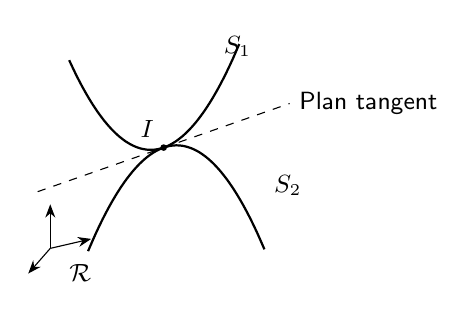
\begin{tikzpicture}[scale=.8]
\draw[thick,domain=-1.5:1.2,smooth,variable=\x] plot (\x,{.35*\x+.85*\x*\x});
\draw[thick,domain=-1.2:1.6,smooth,variable=\x] plot (\x,{.35*\x-.85*\x*\x});
\draw[dashed] (-2,-.7)--(2,.7) node[right]{Plan tangent};
\fill (0,0) circle(1.5pt);\node[above left] at (0,0){$I$};\node[right] at (.8,1.6){$S_1$};\node[right] at (1.6,-.6){$S_2$};
\begin{scope}[shift={(-1.8,-1.6)}]\repere\end{scope}
\end{tikzpicture}}
\begin{document}
{\fontsize{27}{31}\selectfont\bfseries Révisions de mécanique\par}
\vspace{4mm}
\begingroup\setlength{\parskip}{2pt}
\planpart{I}{Système}
\planpart{II}{Grandeurs cinétiques}
\plansub{1)}{Quantité de mouvement}
\plansub{2)}{Moment cinétique}
\plansub{3)}{Énergie cinétique}
\planpart{III}{Bilan des forces}
\planpart{IV}{Lois de la dynamique}
\plansub{1)}{Théorème de la quantité de mouvement}
\plansub{2)}{Théorème du moment cinétique}
\plansub{3)}{Théorème énergétique}
\planpart{V}{Méthode}
\planpart{VI}{Complément : contact ponctuel entre deux solides}
\plansub{1)}{Vitesse de glissement}
\plansub{2)}{Forces de contact}
\plansub{3)}{Puissance totale des actions de contact}
\plansub{4)}{Exemples}
\plansub{5)}{Cas d'absence de glissement}
\plansub{6)}{Cas du glissement}
\endgroup
\vspace{3mm}
% Source : page 1.
\section{Système}
\begin{minipage}{.49\linewidth}\centering
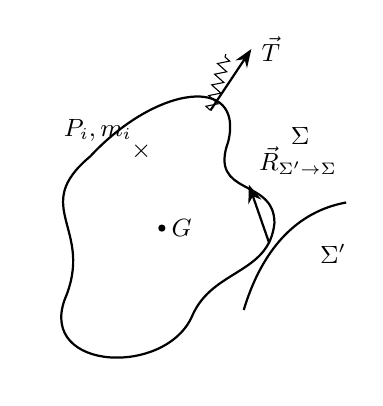
\begin{tikzpicture}[scale=.65]
\draw[thick] (-1.5,1.2)..controls (-2.7,.2) and (-1.4,-.2)..(-2,-1.6)..controls (-2.5,-3) and (0,-3.1)..(.5,-1.9)..controls (.9,-1) and (2,-1.1)..(2.1,-.1)..controls (2.1,.8) and (.8,.4)..(1.2,1.5)..controls (1.5,2.8) and (-.2,2.6)..(-1.5,1.2);
\node at (2.6,1.6){$\Sigma$};\fill (-.1,-.2) circle(2pt) node[right]{$G$};\node at (-.5,1.3){$\times$};\node[above left] at (-.5,1.3){$P_i,m_i$};
\draw[decorate,decoration={zigzag,segment length=4pt,amplitude=2pt}] (.85,2.1)--(1.15,3.2);\draw[flow] (.85,2.1)--(1.65,3.3) node[right]{$\vec T$};
\draw[thick] (1.5,-1.8)..controls (1.8,-.8) and (2.4,.1)..(3.5,.3);\node[right] at (2.8,-.7){$\Sigma'$};\draw[flow] (2,-.5)--(1.6,.65) node[above right]{$\vec R_{\Sigma'\to\Sigma}$};
\end{tikzpicture}
\end{minipage}\hfill
\begin{minipage}{.46\linewidth}
Le système $\Sigma$ est constitué des points $\{P_i,m_i\}$.

$G$ est le centre d'inertie.
\[m_{\mathrm{tot}}=\sum_i m_i.\]
\end{minipage}
\section{Grandeurs cinétiques}
\subsection{Quantité de mouvement}
\[\vec p_{\RR}(\Sigma)=\sum_i m_i\vec v_{\RR}(P_i)=m_{\mathrm{tot}}\vec v_{\RR}(G).\]
\subsection{Moment cinétique}
\[\vec L_{O/\RR}(\Sigma)=\sum_i\overrightarrow{OP_i}\wedge m_i\vec v_{\RR}(P_i).\]
\[L_\Delta=\vec L_{O/\RR}(\Sigma)\cdot\vec u_\Delta.\]
\subsection{Énergie cinétique}
\[K_{\RR}(\Sigma)=\sum_i\frac12m_i v_{\RR}^2(P_i).\]
\section{Bilan des forces}
% Source : pages 1-2.
On distingue les forces intérieures et les forces extérieures. Les forces extérieures comprennent :
\begin{itemize}
\item les forces à distance : interaction gravitationnelle et interaction électromagnétique ;
\item les forces de contact.
\end{itemize}
\section{Lois de la dynamique}
\subsection{Théorème de la quantité de mouvement}
Dans un référentiel galiléen $\RR_g$, le théorème de la quantité de mouvement (TQM) s'écrit :
\[\left.\frac{\dd\vec p_{\RR_g}(\Sigma)}{\dd t}\right|_{\RR_g}=\vec F_{\mathrm{ext}}.\]
\subsection{Théorème du moment cinétique}
Le théorème du moment cinétique (TMC), par rapport au point $O$, s'écrit :
\[\left.\frac{\dd\vec L_{O/\RR_g}}{\dd t}\right|_{\RR_g}=\vec M_O^{\mathrm{ext}}.\]
\textbf{Pensez au bras de levier !}
\begin{center}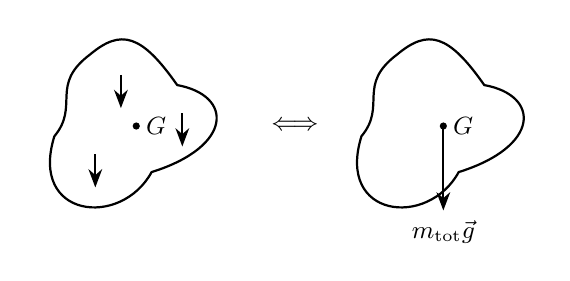
\begin{tikzpicture}[scale=.65]
\foreach \x in {0,6}{\begin{scope}[shift={(\x,0)}]
\draw[thick] (-1,1.4)..controls (-1.8,.8) and (-1.2,.4)..(-1.7,-.2)..controls (-2.2,-1.8) and (-.4,-2)..(.2,-.9)..controls (1.8,-.4) and (1.8,.6)..(.7,.8)..controls (0,1.8) and (-.4,1.9)..(-1,1.4);
\fill (-.1,0) circle(2pt) node[right]{$G$};\end{scope}}
\foreach \x/\y in {-.4/1,-.9/-.55,.8/.25}{\draw[flow] (\x,\y)--+(0,-.65);}
\node at (3,0){$\Longleftrightarrow$};\draw[flow] (5.9,0)--(5.9,-1.65) node[below]{$m_{\mathrm{tot}}\vec g$};
\end{tikzpicture}\end{center}
\textbf{Cette équivalence vaut pour le poids uniquement, pas dans le cas général.}
\[\sum_i m_i\vec g=m_{\mathrm{tot}}\vec g=\vec F_{\mathrm{ext}}^{\mathrm{res}}.\]
\begin{align*}
\vec M_O^{\mathrm{ext}}&=\sum_i\overrightarrow{OP_i}\wedge m_i\vec g
=\left(\sum_i m_i\overrightarrow{OP_i}\right)\wedge\vec g\\
&=m_{\mathrm{tot}}\overrightarrow{OG}\wedge\vec g
=\vec M_O\bigl(\vec F_{\mathrm{ext}}^{\mathrm{res}}\bigr).
\end{align*}
% Source : page 3.
\subsection{Théorème énergétique}
\[\left.\frac{\dd K_{\RR_g}(\Sigma)}{\dd t}\right|_{\RR_g}
=\mathcal P_{\RR_g}^{\mathrm{ext}}+\mathcal P^{\mathrm{int}}.\]
\textbf{Attention aux forces intérieures !} La puissance $\mathcal P^{\mathrm{int}}$ :
\begin{enumerate}
\item est indépendante du référentiel ;
\item est nulle dans un système indéformable.
\end{enumerate}
\section{Méthode}
\begin{enumerate}
\item Définir le système et le référentiel.
\item Déterminer les degrés de liberté.
\item Effectuer le bilan des actions et identifier les grandeurs conservées, par exemple la quantité de mouvement $\vec p_{\RR}$.
\end{enumerate}
\begin{exemple}
\begin{center}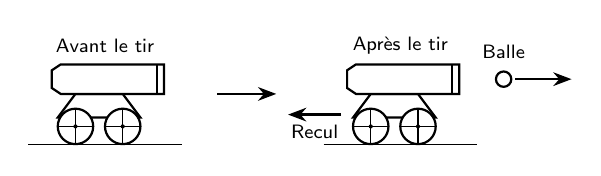
\begin{tikzpicture}[scale=.75]
% Deux états : avant le tir, puis départ de la balle et recul du canon.
\foreach \x in {0,5}{
\begin{scope}[shift={(\x,0)}]
\draw[thin] (-1,-.65)--(1.6,-.65);
\draw[thick,fill=white] (-.5,-.2)--(.9,-.2)--(.6,.2)--(-.2,.2)--cycle;
\draw[thick,fill=white] (-.45,.2)--(-.6,.3)--(-.6,.6)--(-.45,.7)--(1.3,.7)--(1.3,.2)--cycle;
\draw[thick] (1.18,.2)--(1.18,.7);
\foreach \w in {-.2,.6}{
\draw[thick,fill=white] (\w,-.35) circle(.3);
\fill (\w,-.35) circle(1pt);
\draw (\w,-.65)--(\w,-.05);
\draw (\w-.3,-.35)--(\w+.3,-.35);}
\end{scope}}
\node[font=\scriptsize] at (.3,1.02){Avant le tir};
\node[font=\scriptsize] at (5.3,1.02){Après le tir};
\draw[->,thick] (2.2,.2)--(3.2,.2);
\draw[flow] (4.3,-.15)--(3.4,-.15) node[midway,below,font=\scriptsize]{Recul};
\draw[thick,fill=white] (7.05,.45) circle(.13);
\draw[flow] (7.25,.45)--(8.2,.45);
\node[above,font=\scriptsize] at (7.05,.63){Balle};
\end{tikzpicture}\end{center}
\end{exemple}
\begin{exemple}
\begin{minipage}{.43\linewidth}\centering
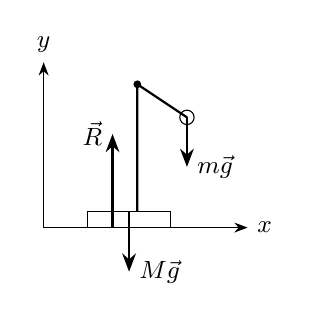
\begin{tikzpicture}[scale=.7]
\draw[->] (-1.7,-1)--(2,-1) node[right]{$x$};\draw[->] (-1.7,-1)--(-1.7,2) node[above]{$y$};
\draw (-.9,-1) rectangle(.6,-.7);\draw[thick] (0,-.7)--(0,1.6)--(.9,1);\fill (0,1.6) circle(2pt);\draw (.9,1) circle(.13);
\draw[flow] (.9,1)--(.9,.1) node[right]{$m\vec g$};\draw[flow] (-.15,-.7)--(-.15,-1.8) node[right]{$M\vec g$};\draw[flow] (-.45,-1)--(-.45,.7) node[left]{$\vec R$};
\end{tikzpicture}
\end{minipage}\hfill\begin{minipage}{.53\linewidth}
La composante $p_x$ est conservée en l'absence de frottements solides.
\end{minipage}
\end{exemple}
% Source : page 4.
\section{Complément : contact ponctuel entre deux solides}
\subsection{Vitesse de glissement}
\begin{minipage}{.42\linewidth}\centering\contact\par Contact ponctuel en $I$.
\end{minipage}\hfill\begin{minipage}{.55\linewidth}
\[\vec v_{g,S_1/S_2}=\vec v_{\RR}(I_1)-\vec v_{\RR}(I_2).\]
\begin{enumerate}
\item $\vec v_{g,S_1/S_2}$ appartient au plan tangent en $I$ à $S_1/S_2$.
\item $\vec v_{g,S_1/S_2}$ est indépendante de $\RR$.
\end{enumerate}
\end{minipage}
\subsection{Forces de contact}
\[\vec R_{1\to2}=-\vec R_{2\to1},\qquad
\vec R_{2\to1}=\vec N_{2\to1}+\vec T_{2\to1}.\]
La réaction normale $\vec N_{2\to1}$ est perpendiculaire au plan tangent $(\pi)$.
La réaction tangentielle $\vec T_{2\to1}$ appartient à $(\pi)$ et correspond aux frottements solides.
\begin{center}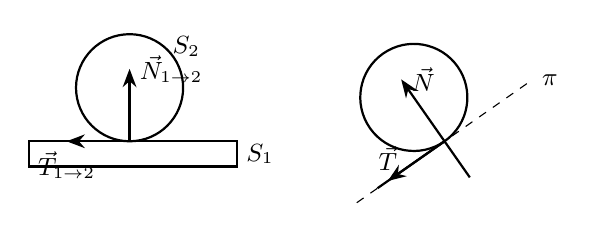
\begin{tikzpicture}[scale=.8]
\draw[thick] (-1.6,-.4) rectangle(1.7,0);\node[right] at (1.7,-.2){$S_1$};\draw[thick] (0,.85) circle(.85);\node at (.9,1.5){$S_2$};
\draw[flow] (0,0)--(0,1.15) node[right]{$\vec N_{1\to2}$};\draw[flow] (0,0)--(-1,0) node[below]{$\vec T_{1\to2}$};
\begin{scope}[shift={(5,0)},rotate=35]
\draw[thick] (-1.3,0)--(0,0)--(0,-.7);\draw[thick] (0,.85) circle(.85);\draw[dashed] (-1.7,0)--(1.7,0) node[right]{$\pi$};
\draw[flow] (0,0)--(0,1.2) node[right]{$\vec N$};\draw[flow] (0,0)--(-1.1,0) node[above]{$\vec T$};
\end{scope}
\end{tikzpicture}\end{center}
% Source : page 5.
\subsection{Puissance totale des actions de contact}
\begin{minipage}{.37\linewidth}\centering\contact\end{minipage}\hfill
\begin{minipage}{.60\linewidth}
Le système étudié est $\{S_1+S_2\}$.
\begin{align*}
\mathcal P_{\mathrm{tot}}&=\vec R_{1\to2}\cdot\vec v_{\RR}(I_2)+\vec R_{2\to1}\cdot\vec v_{\RR}(I_1)\\
&=\vec R_{1\to2}\cdot\vec v_{\RR}(I_2)-\vec R_{1\to2}\cdot\vec v_{\RR}(I_1)\\
&=\vec R_{1\to2}\cdot\bigl(\vec v_{\RR}(I_2)-\vec v_{\RR}(I_1)\bigr)\\
&=\vec R_{1\to2}\cdot\vec v_{g,S_2/S_1}\\
&=(\vec N_{1\to2}+\vec T_{1\to2})\cdot\vec v_{g,S_2/S_1}.
\end{align*}
\end{minipage}
\begin{cadre}[etoiles={\etoiles{3}}]
\[\mathcal P_{\mathrm{tot}}=\vec T_{1\to2}\cdot\vec v_{g,S_2/S_1}.\]
\end{cadre}
En effet, $\vec N_{1\to2}\perp\vec v_{g,S_2/S_1}$.
\begin{cadre}[etoiles={\etoiles{5}}]\textbf{Deux cas importants}\end{cadre}
\begin{enumerate}
\item En l'absence de frottements :
\[\vec T_{1\to2}=\vec0\quad\Longrightarrow\quad\mathcal P_{\mathrm{tot}}=0.\]
\item En l'absence de mouvement relatif :
\[\vec v_{g,S_2/S_1}=\vec0\quad\Longrightarrow\quad\mathcal P_{\mathrm{tot}}=0.\]
\end{enumerate}
% Source : page 6.
\subsection{Exemples}
\begin{exemple}[breakable]
\titr{Exemple 1}
\begin{minipage}{.49\linewidth}\centering
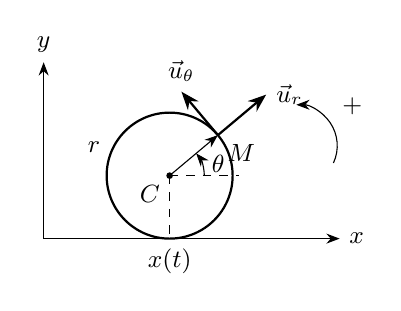
\begin{tikzpicture}[scale=.8]
\draw[->] (-2,-1)--(2.7,-1) node[right]{$x$};\draw[->] (-2,-1)--(-2,1.8) node[above]{$y$};\draw[thick] (0,0) circle(1);
\fill (0,0) circle(1.5pt) node[below left]{$C$};\node[left] at (-.95,.45){$r$};\draw[dashed] (0,0)--(0,-1) node[below]{$x(t)$};
\coordinate (M) at (40:1);\draw[->] (0,0)--(M);\draw[flow] (M)--++(40:1) node[right]{$\vec u_r$};\draw[flow] (M)--++(130:.9) node[above]{$\vec u_\theta$};\node[below right] at (M){$M$};\draw[dashed] (0,0)--(1.1,0);\draw[->] (.55,0) arc(0:40:.55) node[midway,right]{$\theta$};
\draw[->] (2.6,.2) arc(-25:90:.65);\node at (2.9,1.1){$+$};
\end{tikzpicture}
\end{minipage}\hfill\begin{minipage}{.47\linewidth}
Il y a deux degrés de liberté :
\begin{itemize}
\item la rotation, décrite par $\theta(t)$ ;
\item le mouvement horizontal, décrit par $x(t)$.
\end{itemize}
\end{minipage}
\titr{Condition de roulement sans glissement}
\begin{align*}
\vec v_{g,S_2/S_1}&=\vec v_{\RR}(M=I)=\left.\frac{\dd\overrightarrow{OM}}{\dd t}\right|_{\RR}\\
&=\underbrace{\left.\frac{\dd\overrightarrow{OC}}{\dd t}\right|_{\RR}}_{\vec v_{\RR}(C)=\dot x\ux}
+\underbrace{\left.\frac{\dd\overrightarrow{CM}}{\dd t}\right|_{\RR}}_{\frac{\dd}{\dd t}(R\vec u_r)=R\frac{\dd\vec u_r}{\dd t}=R\dot\theta\vec u_\theta}.
\end{align*}
Au point $I$, $\theta=-\dfrac\pi2$ et $\vec u_\theta=\ux$. Ainsi,
\[\vec v_{g,S_2/S_1}=(\dot x+R\dot\theta)\ux.\]
La condition de non-glissement est donc :
\begin{cadre}[etoiles={\etoiles{3}}]\[\dot x=-R\dot\theta.\]\end{cadre}
\textbf{Remarque :} pour $\dot x>0$, on a $\dot\theta<0$, ce qui est cohérent.
\titr{Retour sur la puissance}
\begin{align*}
\mathcal P_{\mathrm{tot}}&=\mathcal P_{\RR}(\vec R_{1\to2})+\underbrace{\mathcal P_{\RR}(\vec R_{2\to1})}_{=0\text{ car }S_1\text{ est fixe}}\\
&=\vec R_{1\to2}\cdot\vec v_{\RR}(I_2).
\end{align*}
La force $\vec R_{1\to2}$ ne travaille pas s'il y a roulement sans glissement.
\end{exemple}
\begin{exemple}
\titr{Exemple 2}
\begin{minipage}{.41\linewidth}\centering
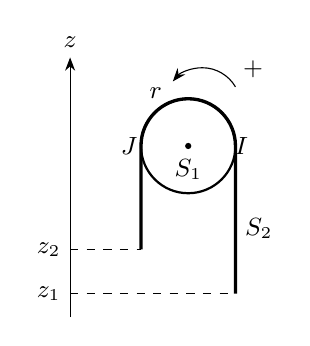
\begin{tikzpicture}[scale=.75]
\draw[->] (-2,-2.4)--(-2,2) node[above]{$z$};\draw[thick] (0,.5) circle(.8);\fill (0,.5) circle(1.5pt);\node at (0,.1){$S_1$};\node at (.9,.5){$I$};\node at (-1,.5){$J$};\node at (-.55,1.4){$r$};
\draw[very thick] (-.8,-1.25)--(-.8,.5) arc(180:0:.8)--(.8,-2);\node[right] at (.8,-.9){$S_2$};\draw[dashed] (-2,-1.25)--(-.8,-1.25);\draw[dashed] (-2,-2)--(.8,-2);\node[left] at (-2,-1.25){$z_2$};\node[left] at (-2,-2){$z_1$};\draw[->] (.8,1.5) arc(30:140:.65);\node at (1.1,1.8){$+$};
\end{tikzpicture}
\end{minipage}\hfill\begin{minipage}{.56\linewidth}
Le système est $S_1+S_2$ et $\mathcal P_{\mathrm{tot}}=0$.

Les conditions de non-glissement sont :
\[\dot z_1=R\dot\theta,\qquad\dot z_2=-R\dot\theta.\]
\end{minipage}
\end{exemple}
% Source : page 7.
\begin{exemple}
\titr{Exemple 3}
\begin{minipage}{.38\linewidth}\centering
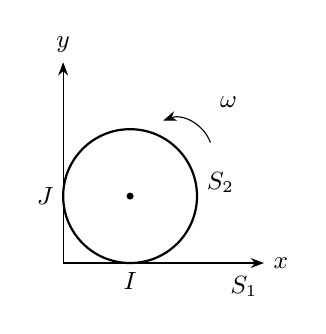
\begin{tikzpicture}[scale=.85]
\draw[->] (-1,-1)--(2,-1) node[right]{$x$};\draw[->] (-1,-1)--(-1,2) node[above]{$y$};\draw[thick] (0,0) circle(1);\fill (0,0) circle(1.5pt);\node[right] at (1,.2){$S_2$};\node at (1.7,-1.35){$S_1$};\node[left] at (-1,0){$J$};\node[below] at (0,-1){$I$};\draw[->] (1.2,.8) arc(20:110:.55);\node[right] at (1.2,1.4){$\omega$};
\end{tikzpicture}\par $\RR=(Oxyz)$.
\end{minipage}\hfill\begin{minipage}{.59\linewidth}
Il y a glissement relatif en $I$ et $J$.
\begin{align*}
\text{En }I:\quad\vec v_{g,S_2/S_1}&=\vec v_{\RR}(I_2)-\vec v_{\RR}(I_1)\\
&=\vec v_{\RR}(I_2)\\
&=R\omega(t)\ux.
\end{align*}
\[\text{En }J:\quad\vec v_{g,S_2/S_1}=-R\omega(t)\uy.\]
\end{minipage}
\end{exemple}
\par\medskip
\begin{minipage}{.28\linewidth}\centering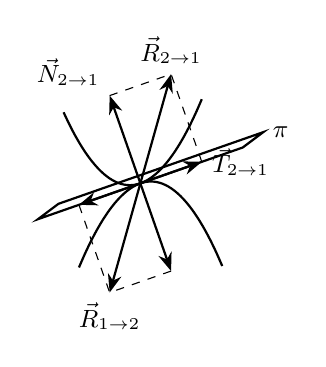
\begin{tikzpicture}[scale=.65]
\draw[thick,domain=-1.5:1.2,smooth,variable=\x] plot (\x,{.35*\x+.85*\x*\x});
\draw[thick,domain=-1.2:1.6,smooth,variable=\x] plot (\x,{.35*\x-.85*\x*\x});
\draw[thick] (-2,-.7)--(2,.7)--(2.4,1)--(-1.6,-.4)--cycle;\node[right] at (2.4,1){$\pi$};
\draw[flow] (0,0)--(-.6,1.714) node[above left]{$\vec N_{2\to1}$};
\draw[flow] (0,0)--(1.2,.42) node[right]{$\vec T_{2\to1}$};
\draw[flow] (0,0)--(.6,2.134) node[above]{$\vec R_{2\to1}$};
\draw[dashed] (-.6,1.714)--(.6,2.134)--(1.2,.42);
\draw[flow] (0,0)--(-.6,-2.134) node[below]{$\vec R_{1\to2}$};
\draw[flow] (0,0)--(.6,-1.714);\draw[flow] (0,0)--(-1.2,-.42);\draw[dashed] (.6,-1.714)--(-.6,-2.134)--(-1.2,-.42);
\end{tikzpicture}\end{minipage}\hfill
\begin{minipage}{.69\linewidth}
\subsection{Cas d'absence de glissement}
\[\vec v_{g,1/2}=\vec0.\]
\begin{cadre}[etoiles={\etoiles{3}}]
\[\|\vec T_{2\to1}\|<f_s\|\vec N_{2\to1}\|.\]
\end{cadre}
$f_s$ est le coefficient de frottement statique.
\subsection{Cas du glissement}
\[\vec v_{g,1/2}\ne\vec0.\]
\begin{cadre}
\[\|\vec T_{2\to1}\|=f_D\|\vec N_{2\to1}\|.\]
$\vec T_{2\to1}$ est anticolinéaire à $\vec v_{g,1/2}$.
\end{cadre}
% Source : pages 7-8.
\begin{cadre}[etoiles={\etoiles{3}}]
\[\vec T_{2\to1}=-f_D\|\vec N_{2\to1}\|\frac{\vec v_{g,1/2}}{\|\vec v_{g,1/2}\|}.\]
\end{cadre}
\end{minipage}
\end{document}